\documentclass[a4j,12pt,]{jarticle}
 \usepackage{float}
 \usepackage{siunitx} %%SI単位系用
 \usepackage{amssymb, amsmath}
 \usepackage{ascmac,here,txfonts}
 \usepackage{hyperref}
 \usepackage{listings}
 \usepackage{pxjahyper}
 \usepackage[dvipdfmx]{graphicx}
 \usepackage{amssymb, amsmath}
  \usepackage{listings}
  \usepackage[dvipdfmx]{color}

  \lstset{
    language={Python},
    basicstyle={\ttfamily},
    identifierstyle={\small},
    commentstyle={\small\itshape},
    keywordstyle={\small\bfseries},
    ndkeywordstyle={\small},
    stringstyle={\small\ttfamily},
    frame={single},
    breaklines=true,
    columns=[l]{fullflexible},
    numbers=left,
    xrightmargin=0zw,
    xleftmargin=3zw,
    numberstyle={\scriptsize},
    stepnumber=1,
    numbersep=1zw,
    lineskip=-0.5ex,
  }

\begin{document}

{\noindent\small 第20回報告書 \hfill\today}
\begin{center}
  {\Large 異なるバージョンの Elasticsearch ノードのクラスタリング}
\end{center}
\begin{flushright}
  祖父江匠真 \\
\end{flushright}

\section{概要}
今回は, Docker Compose を使用して, 異なるバージョンである7.17.6 と 7.17.9 の Elasticsearch ノードをクラスタリングすることが可能かどうかを確認するために実施した実験について説明する.

クラスタの構築には, Docker Composeを使用した.

\section{Dockerとは}
Dockerは, アプリケーションをコンテナと呼ばれる隔離された環境で実行するためのツールである. コンテナは軽量で, システムリソースを共有し, それぞれが独自のファイルシステム, プロセス空間, メモリなどを持っている. これにより, 異なる環境で同じアプリケーションを一貫して実行できる.

\section{Docker Composeとは}
Docker Composeは, 複数のコンテナを定義し, 実行するためのツールである. これはYAMLファイルを使用して設定され, 複数のコンテナを使用したシステムの構築を単純化する.

\section{実験セットアップ}
\subsection{全て同じバージョンのElasticSearchを使用したクラスタ構成 (全ノード バージョン 7.17.9)}

Listing \ref{sc1}にクラスタを構成するのに使用したdocker-compose.ymlファイルの内容を記載する.

\begin{lstlisting}[caption=全て同じバージョンのElasticSearchを使用したクラスタを構成するdocker-compose.yml, label=sc1]
version: '2.2'
services:
  es01:
    image: docker.elastic.co/elasticsearch/elasticsearch:7.17.9
    container_name: es01
    environment:
      - node.name=es01
      - cluster.name=es-docker-cluster
      - discovery.seed_hosts=es02,es03
      - cluster.initial_master_nodes=es01,es02,es03
      - bootstrap.memory_lock=true
      - "ES_JAVA_OPTS=-Xms2048m -Xmx2048m"
    ulimits:
      memlock:
        soft: -1
        hard: -1
    volumes:
      - data01:/usr/share/elasticsearch/data
    ports:
      - 9200:9200
    networks:
      - elastic
  es02:
    image: docker.elastic.co/elasticsearch/elasticsearch:7.17.9
    container_name: es02
    environment:
      - node.name=es02
      - cluster.name=es-docker-cluster
      - discovery.seed_hosts=es01,es03
      - cluster.initial_master_nodes=es01,es02,es03
      - bootstrap.memory_lock=true
      - "ES_JAVA_OPTS=-Xms2048m -Xmx2048m"
    ulimits:
      memlock:
        soft: -1
        hard: -1
    volumes:
      - data02:/usr/share/elasticsearch/data
    networks:
      - elastic
  es03:
    image: docker.elastic.co/elasticsearch/elasticsearch:7.17.9
    container_name: es03
    environment:
      - node.name=es03
      - cluster.name=es-docker-cluster
      - discovery.seed_hosts=es01,es02
      - cluster.initial_master_nodes=es01,es02,es03
      - bootstrap.memory_lock=true
      - "ES_JAVA_OPTS=-Xms2048m -Xmx2048m"
    ulimits:
      memlock:
        soft: -1
        hard: -1
    volumes:
      - data03:/usr/share/elasticsearch/data
    networks:
      - elastic

volumes:
  data01:
    driver: local
  data02:
    driver: local
  data03:
    driver: local

networks:
  elastic:
    driver: bridge
\end{lstlisting}

Listing \ref{sc1}のdocker-compose.ymlファイルで記述している内容について説明する.

\subsubsection*{サービスの定義}
\begin{itemize}
  \item \textbf{es01, es02, es03}: これらはElasticsearchのノード(サーバー)である. 各ノードは異なるコンテナとして定義されている. `es01`, `es02`, `es03`はそれぞれ異なるコンテナ名で, Elasticsearchの異なるインスタンスを実行する.
\end{itemize}

\subsubsection*{各ノードの設定}
\begin{itemize}
  \item \textbf{image}: 使用するDockerイメージ。ここではElasticsearchの7.17.9バージョンを使用している. 
  \item \textbf{container\_name}: コンテナに割り当てられる名前。
  \item \textbf{environment}: 環境変数の設定。Elasticsearchのクラスタ設定, メモリ設定などを含みます。
  \item \textbf{ulimits}: メモリロックの限界を設定。これによりElasticsearchがメモリを効率的に利用できる.
  \item \textbf{volumes}: データ永続化のためのボリュームマウント。データをコンテナの外に保存する.
  \item \textbf{ports}: ホストマシンとコンテナ間のポートマッピング。例えば, `9200:9200`はホストの9200ポートをコンテナの9200ポートにマッピングする.
  \item \textbf{networks}: コンテナ間通信のためのネットワーク設定。ここでは`elastic`ネットワークが使用されている. 
\end{itemize}

\subsubsection*{ボリュームとネットワークの設定}
\begin{itemize}
  \item \textbf{volumes}: `data01`, `data02`, `data03`はデータの永続化に使用されるボリュームである. これによりコンテナが削除されてもデータが保持される.
  \item \textbf{networks}: `elastic`ネットワークはブリッジドライバを使用している. これにより, 異なるコンテナが相互に通信できるようになる.
\end{itemize}

この設定により, Elasticsearchの3ノードを含むクラスタがDocker上で動作するようセットアップされる.

クラスタの起動には, docker compose up -dコマンドを使用する.

docker compose up -dコマンドを実行した後, curlコマンドを使用してクラスタに参加しているノードを一覧表示した結果を図 \ref{p1}に示す.

\begin{figure}[H]
  \begin{center}
    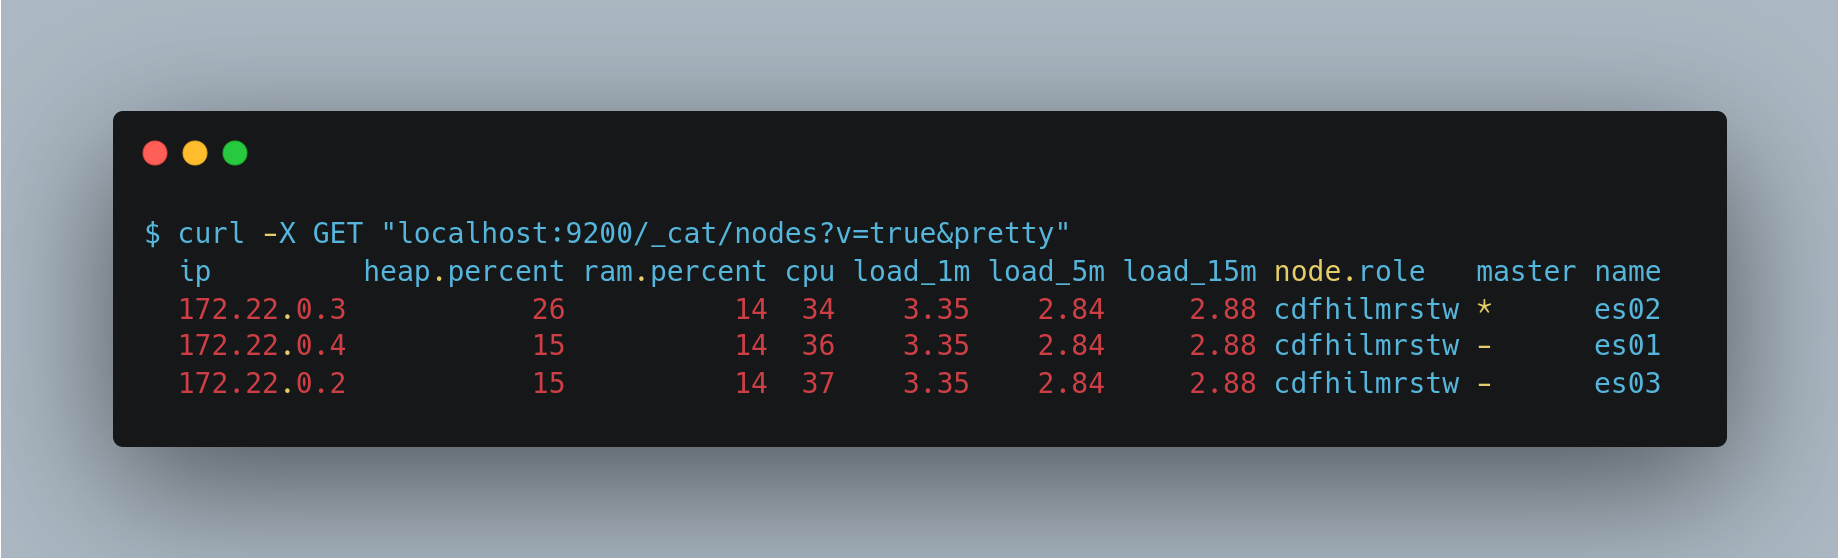
\includegraphics[width=160mm]{curl-same.png}
    \caption{クラスタに参加しているノードを一覧表示した結果}
    \label{p1}
  \end{center}
\end{figure}

% \begin{lstlisting}[caption=クラスタに参加しているノードを一覧表示した結果, label=re1]
% $ curl -X GET "localhost:9200/_cat/nodes?v=true&pretty"
%   ip         heap.percent ram.percent cpu load_1m load_5m load_15m node.role   master name
%   172.22.0.3           26          14  34    3.35    2.84     2.88 cdfhilmrstw *      es02
%   172.22.0.4           15          14  36    3.35    2.84     2.88 cdfhilmrstw -      es01
%   172.22.0.2           15          14  37    3.35    2.84     2.88 cdfhilmrstw -      es03
% \end{lstlisting}

図 \ref{p1}より, 3つのノード(`es01`, `es02`, `es03`)すべてが正常にクラスタに参加できていることが確認できる.

\subsection{異なるバージョンのElasticSearchを使用したクラスタ構成 (2ノード バージョン 7.17.9, 1ノード バージョン 7.17.6)}

Listing \ref{sc1}のdocker-compose.ymlをListing \ref{sc2}のように変更することで, es03のノードで使用するElasticSearchのバージョンを7.17.9から7.17.6に変更する.

\begin{lstlisting}[caption=Listing \ref{sc1}のdocker-compose.ymlから変更を加えた箇所, label=sc2]
version: '2.2'
services:
  ...
  es03:
    image: docker.elastic.co/elasticsearch/elasticsearch:7.17.6
    ...

...
\end{lstlisting}

変更後, docker compose up -dコマンドを実行してクラスタを起動する.

クラスタの起動後, curlコマンドを使用してクラスタに参加しているノードを一覧表示した結果を図 \ref{p2}に示す.

\begin{figure}[H]
  \begin{center}
    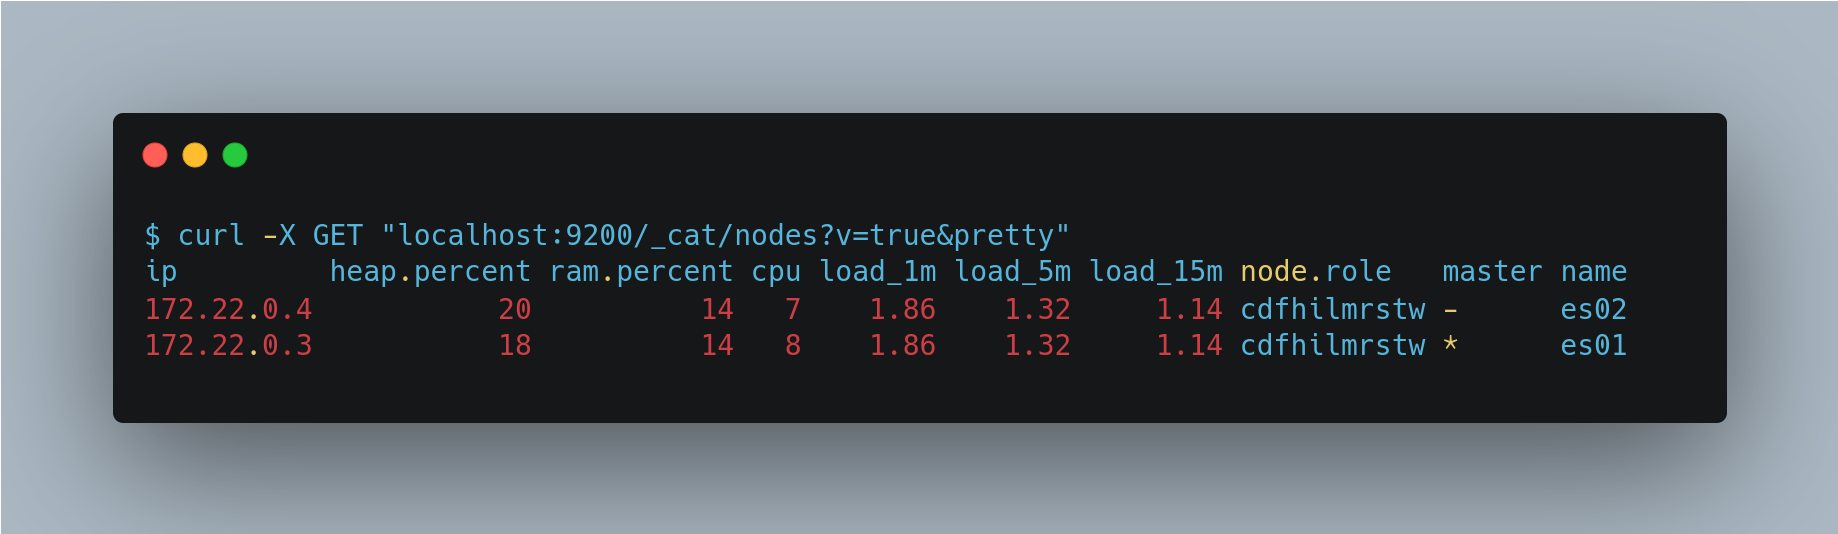
\includegraphics[width=160mm]{curl-different.png}
    \caption{クラスタに参加しているノードを一覧表示した結果}
    \label{p2}
  \end{center}
\end{figure}

図 \ref{p2}より, バージョンが7.17.9である2つのノード(`es01`, `es02`)のみが正常にクラスタに参加できていることが確認できる.

\section{まとめ}
今回は, Docker Compose を使用して, 異なるバージョンである7.17.6 と 7.17.9 の Elasticsearch ノードをクラスタリングすることが可能かどうかを確認した.

今回の実験により, Docker Compose を使用した Elasticsearch ノードのクラスタリングは, 全てのノードが同じバージョンであれば行えることが実証された. しかし, 異なるマイナーバージョン(今回は7.17.6と7.17.9)のノードをクラスタ化しようとすると, 古いバージョンのノードはクラスタに参加できなかった.

そのため, サーバーゾーンでのリサイクル館の測定データを保存しているElasticSearchをバージョンアップする必要があり, 次回はElasticSearchのバージョンアップ方法について調査した結果を報告する.

\begin{thebibliography}{5}
  \bibitem{1}Elasticsearch B.V., ”Install Elasticsearch with Docker | Elasticsearch Guide [7.17] | Elastic”, https://www.elastic.co/guide/en/elasticsearch/reference/7.17/docker.html, 参照 Nov 17,2023.
\end{thebibliography}

\end{document}

